\subsection{Diagrama de Estados}
\label{subsec:diagrama_estados_quejoso}

El ciclo de vida de una queja dentro del sistema se gestiona mediante el siguiente diagrama de estados desde la perspectiva del quejoso. Este modelo tiene el fin de mostrar cómo determina qué acciones (como editar o eliminar) están habilitadas en su tablero de control según la etapa administrativa en la que se encuentre su expediente.

El tablero del quejoso refleja cinco estados principales, los cuales son mostrados en el diagrama y explicados a continuación:

\begin{itemize}
    \item \textbf{RECIBIDA:} Estado inicial donde el quejoso mantiene el control total para editar o eliminar su registro.
    \item \textbf{EN REVISIÓN:} Fase de análisis administrativo por la Defensoría donde el expediente queda en modo de solo lectura.
    \item \textbf{ASIGNADA\_DEFENSOR:} Etapa de mediación que requiere una decisión vinculante (aceptar o rechazar) por parte del quejoso.
    \item \textbf{CONCLUIDA:} Estado final que habilita la descarga de la resolución y el cierre del expediente.
    \item \textbf{CANCELADA:} Estado final alcanzado únicamente cuando el quejoso decide eliminar la queja antes de su admisión.
\end{itemize}

\begin{figure}[H]
    \centering
    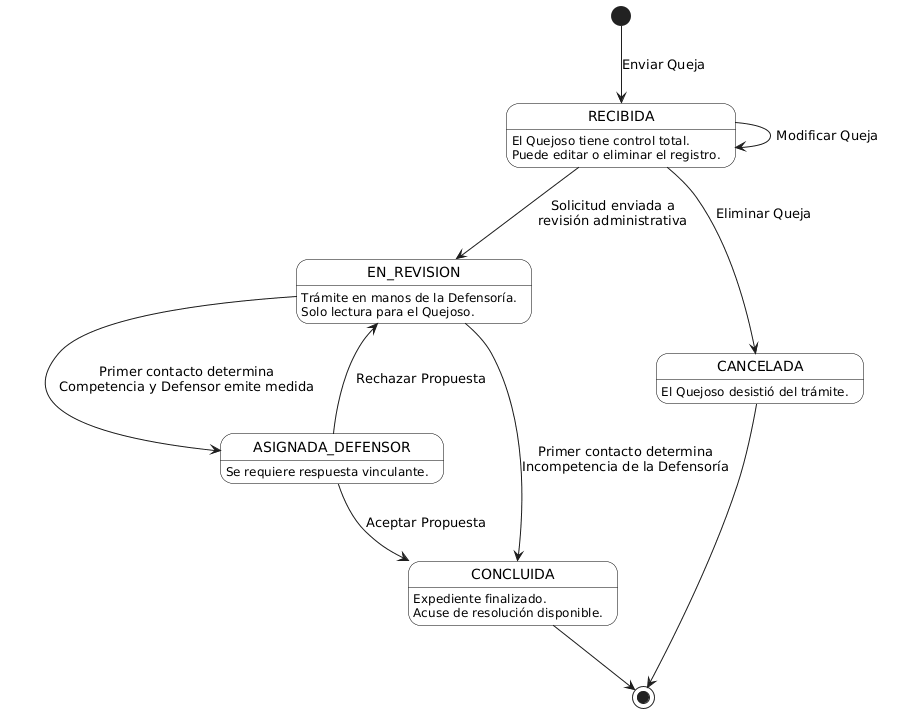
\includegraphics[width=0.82\textwidth, height=0.75\textheight, keepaspectratio]{imagenes/quejoso/D_Estados/DE01-EstadosVistaQuejoso.png}
    \caption{Diagrama de Estados: Ciclo de vida de la Queja}
    \label{fig:de01_estados_quejoso}
\end{figure}
